\documentclass{beamer}
\usetheme[deutsch]{KIT}

\usepackage[utf8]{inputenc}
\usepackage[T1]{fontenc}
\usepackage{listings}
\usepackage{pgfplots}
\usepackage{babel}
\usepackage{tikz,calc,ifthen}
\usepackage{mathtools}
\usepackage[normalem]{ulem}
\usepackage{graphicx}
\usepackage{subfig}
\usepackage{booktabs}
\usepackage{pgfplotstable}

% Colors
\definecolor{firmBlue}     {rgb}{0.6,  0.6, 1   }
\definecolor{firmCyan}     {rgb}{0.8,  1,   1   }
\definecolor{firmDarkBlue} {rgb}{0.4,  0.4, 1   }
\definecolor{firmGreen}    {rgb}{0.42, 1,   0.42}
\definecolor{firmDarkGreen}{rgb}{0,    0.5, 0   }
\definecolor{firmRed}      {rgb}{1,    0.6, 0.6 }
\definecolor{firmViolet}   {rgb}{0.5,  0,   0.5}
\definecolor{firmYellow}   {rgb}{1,    1,   0.6 }

% Nodes
\tikzstyle{graph}      = [fill=lightgray]
\tikzstyle{firm}       = [draw, fill=white]
\tikzstyle{block}      = [draw, fill=yellow]
\tikzstyle{const}      = [draw, fill=firmCyan]
\tikzstyle{control}    = [draw, fill=firmRed]
\tikzstyle{memory}     = [draw, fill=firmBlue]
\tikzstyle{phi}        = [draw, fill=green]
\tikzstyle{proj}       = [draw, fill=firmYellow]
\tikzstyle{start}      = [draw, fill=firmDarkBlue]

% Edges
\tikzstyle{dataDependency}    = [thick, -latex]
\tikzstyle{controlDependency} = [dataDependency, color=red]
\tikzstyle{memoryDependency}  = [dataDependency, color=firmDarkBlue]
\tikzstyle{keep}              = [dataDependency, color=firmViolet]
\tikzstyle{dependency}        = [dataDependency, color=firmDarkGreen]


\usetikzlibrary{positioning,calc,arrows,shapes}
\tikzset{
  every node/.style={transform shape},
  auto,
  block/.style={align=center,rectangle,draw,minimum height=20pt,minimum width=30pt},
  >=triangle 60,
  alt/.code args={<#1>#2#3}{%
      \alt<#1>{\pgfkeysalso{#2}}{\pgfkeysalso{#3}}
  },
  beameralert/.style={alt=<#1>{color=green!80!black}{}},
  mythick/.style={line width=1.4pt}
}

\newcommand*{\maxwidthofm}[2]{\maxof{\widthof{$#1$}}{\widthof{$#2$}}}
\newcommand<>*{\robustaltm}[2]{
  \alt#3
  {\mathmakebox[\maxwidthofm{#1}{#2}]{#1}\vphantom{#1#2}}
    {\mathmakebox[\maxwidthofm{#1}{#2}]{#2}\vphantom{#1#2}}
}

\newcommand<>*{\nodealert}[1]{\only#2{\draw[overlay,mythick,color=green!80!black] (#1.north west) rectangle (#1.south east)}}

\title{Improved integer conversion optimisation and VHDL code generation based on bit-width analysis}
\author{Marcel Hollerbach}
\subtitle{\insertauthor}
\institute[IPD]{Lehrstuhl Programmierparadigmen, IPD Snelting}
\date{29.10.2018}
\KITtitleimage{cover.png}

\begin{document}

\begin{frame}
  \maketitle
\end{frame}


\begin{frame}[fragile]{Das Ziel}
\begin{lstlisting}
int arr[4];

for (int i = 0; i < 4; i++) {

	int x = i*i;      
	int y = (i << 4); 
	int res = x + y;  
	arr[i] = res;
}
\end{lstlisting}
Wie viele bits nutzen \textit{i}, \textit{x}, \textit{y}, \textit{res}? \newline
\end{frame}

\begin{frame}{Was ist eine Bitbreite}
\begin{center}
	\begin{definition}{bitbreite}
		(stable\_bits, is\_positive)
	\end{definition}
\end{center}

\begin{tabular}{ c c | c c c c c c c c | c c }
	mode & value & \multicolumn{8}{c|}{bit representation} & stable\_bits & is\_positive \\
	\hline
	\hline
	Bs & 5     & \color{red}0 & \color {red}0 & \color{red}0 & \color{red}0 & 0 & 1 & 0 & 1 & 4 & true\\
	Bs & -2    & \color{red}1 & \color{red}1 & \color{red}1 & \color{red}1 & \color{red}1 & \color{red}1 & 1 & 0 & 6 & false\\
    Bu & 5     & \color{red}0 & \color{red}0 & \color{red}0 & \color{red}0 & \color{red}0 & 1 & 0 & 1 & 5 & - \\
\end{tabular}

\end{frame}

%\begin{frame}[fragile]{Das Ziel}
%\begin{lstlisting}
%\begin{tabular}{ c c }
%Variable & Verbrauch \\
%i & 3 \\
%x & 6 \\
%y & 7 \\
%res & 8 \\
%\end{tabular}
%\end{lstlisting}
%\end{frame}

\begin{frame}{libFIRM}
\begin{columns}
	\begin{column}{0.5\textwidth}
		\begin{enumerate}
			\item Integer-modes sind genutzt
			\item Nutzung von Arithmetische/Logische ausdruecke
			\item Behandlung von Confirm knoten
		\end{enumerate}
	\end{column}
		\begin{column}{0.5\textwidth}  %%<--- here
			\begin{center}
				\begin{tikzpicture}
				\node[graph]{
					\begin{tikzpicture}[remember picture]
					\node[block] (startblock) {
						\begin{tikzpicture}
						\node[firm]    (const0) at (0,2) {Const : 0};
						\node[phi]     (phi)    at (-1,1) {Phi};
						\node[firm]    (const1) at (1,1) {Const : 1};
						\node[firm]    (add)    at (0,0) {Add};
						\node[firm]    (cmp)        at ( 0,-1) {Cmp less\_equal};
						\node[control] (cond)       at ( 0,-2) {Cond};
						\node[control] (false)      at (-1,-3) {False};
						\node[control] (true)       at ( 1,-3) {True};
						
						\draw[dataDependency]    (add.60)      -- ++(0,0.1) -| (const1);
						\draw[dataDependency]    (add.120)     -- ++(0,0.1) -| (phi);
						\draw[dataDependency]    (phi.60)      -- ++(0,0.1) -| (const0);
						\draw[dataDependency]    (phi.120)     -- ++(0,0.1) -- ++(-1,0) -- ++(0,-2) -| (add.240);
						\draw[dataDependency]    (cmp.62)     --              (add.300);
						\draw[dataDependency]    (cond)        --              (cmp);
						\draw[controlDependency] (false.north) -- ++(0,0.1) -| (cond.240);
						\draw[controlDependency] (true.north)  -- ++(0,0.1) -| (cond.300);
						
						\end{tikzpicture}
					};
				\end{tikzpicture}
			};
		\end{tikzpicture}
		\end{center}
	\end{column}
\end{columns}
\end{frame}

\begin{frame}{libFIRM}
\begin{columns}
	\begin{column}{0.5\textwidth}
		Confirm-node
		\newline
		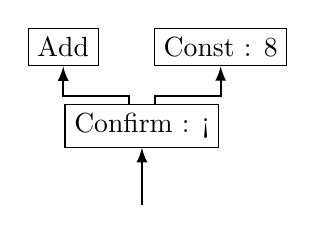
\begin{tikzpicture}
			\node[firm]    (add)    at (-1,1) {Add};
			\node[firm]    (const0) at (1,1) {Const : 8};
			\node[firm]    (confirm) at (0,0) {Confirm : <};
			\draw[dataDependency]    (confirm.60)      -- ++(0,0.1) -| (const0);
			\draw[dataDependency]    (confirm.120)     -- ++(0,0.1) -| (add);
			\draw[dataDependency]    (0,-1) -- (confirm);
		\end{tikzpicture}
		%FIXME
	\end{column}
	\begin{column}{0.5\textwidth}  %%<--- here
		Convertion-node
		\newline
		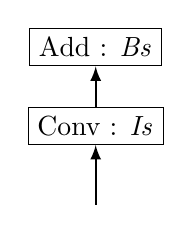
\begin{tikzpicture}
		\node[firm]    (add)    at (0,1) {Add : \textit{Bs}};
		\node[firm]    (conv) at (0,0) {Conv : \textit{Is}};
		\draw[dataDependency]    (conv) -- (add);
		\draw[dataDependency]    (0,-1) -- (conv);
		\end{tikzpicture}
		%FIXME
	\end{column}
\end{columns}
\end{frame}



\begin{frame}{Analyse}
Implementiert mit worklist appraoch.
\begin{center}
	\begin{tabular}{ l | c }
		op & stable bits \\
		\hline
		add & $max(min(a_{stable}, b_{stable}) - 1, 0)$ \\
		minus &  $max(a_{stable} - 1, 0) $ \\
		sub &  $max(min(a_{stable}, b_{stable}) - 1, 0) $ \\
		mul &  $max(2*mode - ( b_{stable} + a_{stable} ), 0)  $ \\
		div &  
		$ 
		\left\{
		\begin{array}{l}
		a_{stable}\\ 
		max(a_{stable} - 1, 0)
		\end{array}
		\begin{array}{l}
		, \neg mode\text{ is signed} \\ 
		, \text{otherwise}.
		\end{array}
		\right.$\\
		mod & 
		$
		\lfloor log2(max(a))\rfloor
		$
		\\
	\end{tabular}
\end{center}
\end{frame}

\begin{frame}{Analyse 2}
\begin{center}
	$add(const(5), x) \equiv max(min(4, 5) - 1, 0) \equiv 3$
\newline
\newline
\newline
\begin{tabular}{ c | c c }
	stable\_bits & min & max \\
	\hline
	\hline
	5 & -4 & +3 \\
	4 & -8 & +7\\
	3 & -16 & +15 \\
\end{tabular}
\end{center}
\end{frame}

\begin{frame}{Schleifen im Graphen}
Mit moeglichem Confirm:
\begin{tikzpicture}
\node[graph]{
	\begin{tikzpicture}[remember picture]
	\node[block] (startblock) {
		\begin{tikzpicture}
		\node[firm]    (const0) at (1,2) {Const : 0};
		\node[phi]     (phi)    at (-1,1) {Phi};
		\node[firm]    (cmp)        at ( 0,-1) {Cmp less\_equal};
		\node[control] (cond)       at ( 0,-2) {Cond};
		\node[control] (false)      at ( 1,-3) {False};
		\node[control] (true)       at (-1,-3) {True};
		
		\draw[dataDependency]    (phi.60)      -- ++(0,0.1) -| (const0);
		\draw[dataDependency]    (cmp.60)        -- ++(0,0.1) -| (phi.300);
		\draw[dataDependency]    (cond)        --              (cmp);
		\draw[controlDependency] (false.north) -- ++(0,0.1) -| (cond.300);
		\draw[controlDependency] (true.north)  -- ++(0,0.1) -| (cond.240);
		\end{tikzpicture}
	};
	\node[block, anchor=east] (end) at ($(startblock.west) + (-1,0)$) {
		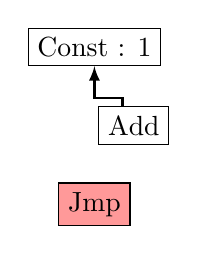
\begin{tikzpicture}
		\node[firm]    (const1) at (0,0) {Const : 1};
		\node[firm]    (add) at (0.5,-1) {Add};
		\node[control] (ret) at (0,-2) {Jmp};
		
		
		\draw[dataDependency] (add.120) -- ++(0,0.1) -| (const1);
		\end{tikzpicture}
	};
	\begin{scope}									
		\draw[dataDependency] (add.60) -- ++(0,0.1) -| (phi);
		\draw[dataDependency]  (phi)-- ++(0,+0.49) -- ++(-4.5,0) -- ++(0,-2.5) -| (add.240);
	\end{scope}
	
	
\end{tikzpicture}
};	
\end{tikzpicture}
\end{frame}


\begin{frame}{Schleifen im Graphen}
Ohne moegliches Confirm:
\begin{tikzpicture}
	\node[graph]{
		\begin{tikzpicture}[remember picture]
			\node[block] (startblock) {
				\begin{tikzpicture}
				\node[firm]    (const0) at (1,2) {Const : 0};
				\node[phi]     (phi)    at (-1,1) {Phi};
				\node[firm]    (conv)    at (0,0) {Conv};
				\node[firm]    (cmp)        at ( 0,-1) {Cmp less\_equal};
				\node[control] (cond)       at ( 0,-2) {Cond};
				\node[control] (false)      at ( 1,-3) {False};
				\node[control] (true)       at (-1,-3) {True};
				
				\draw[dataDependency]    (phi.60)      -- ++(0,0.1) -| (const0);
				\draw[dataDependency]    (conv.60)        -- ++(0,0.1) -| (phi.300);
				\draw[dataDependency]    (cmp)     --              (conv);
				\draw[dataDependency]    (cond)        --              (cmp);
				\draw[controlDependency] (false.north) -- ++(0,0.1) -| (cond.300);
				\draw[controlDependency] (true.north)  -- ++(0,0.1) -| (cond.240);
				\end{tikzpicture}
			};
			\node[block, anchor=east] (end) at ($(startblock.west) + (-1,0)$) {
				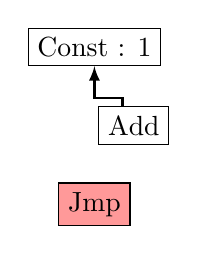
\begin{tikzpicture}
				\node[firm]    (const1) at (0,0) {Const : 1};
				\node[firm]    (add) at (0.5,-1) {Add};
				\node[control] (ret) at (0,-2) {Jmp};
				

				\draw[dataDependency] (add.120) -- ++(0,0.1) -| (const1);
				\end{tikzpicture}
			};
			\begin{scope}									
				\draw[dataDependency] (add.60) -- ++(0,0.1) -| (phi);
				\draw[dataDependency]  (phi)-- ++(0,+0.49) -- ++(-4.5,0) -- ++(0,-2.5) -| (add.240);
			\end{scope}


		\end{tikzpicture}
	};	
\end{tikzpicture}
\end{frame}

\begin{frame}{Zusätzliches Confirm Analyse Ergebnisse}
\begin{columns}
	\begin{column}{0.5\textwidth}
		Stable bits von add:
		\begin{enumerate}
			\item (32, true)
			\item (30, true)
			\item (29, true)
			\item (28, true) [7,-8]
			\item \color{red}(27, true) [15,-16] -> \color{darkgray}insert Confirms
		\end{enumerate}
	\end{column}
	\begin{column}{0.5\textwidth}  %%<--- here
	\begin{tikzpicture}
		\node[graph]{
			\begin{tikzpicture}[remember picture]
				\node[block] (startblock) {
					\begin{tikzpicture}
						\node[firm]    (const0) at (0.5,2) {Const : 0};
						\node[phi]     (phi)    at (-0.4,1) {Phi};
						\node[firm]    (conv)    at (0,0) {Conv};
						\node[firm]    (const2)      at (2,0) {Const : 10};
						\node[firm]    (cmp)        at ( 0,-1) {Cmp less\_equal};
						\node[control] (cond)       at ( 0,-2) {Cond};
						\node[control] (false)      at ( 1,-3) {False};
						\node[control] (true)       at (-1,-3) {True};
						
						\draw[dataDependency]    (phi.60)      --  ++(0,0.1) -| (const0);
						\draw[dataDependency]    (conv.120)        --  ++(0,0.1) -| (phi.300);
						\draw[dataDependency]    (-2.0,0.34)        --  ++(0,0.0) -| (phi.240);
						\draw[thick]             (-2.0,1.45)        --  ++(0,0.0) -| (phi.120);
						\draw[dataDependency]    (cmp)     --              (conv);
						\draw[dataDependency]    (cmp.60)     --    ++(0,0.1)-| (const2);
						\draw[dataDependency]    (cond)        --              (cmp);
						\draw[controlDependency] (false.north) -- ++(0,0.1) -| (cond.300);
						\draw[controlDependency] (true.north)  -- ++(0,0.1) -| (cond.240);
					\end{tikzpicture}
				};
			\end{tikzpicture}
		};	
	\end{tikzpicture}
	\end{column}
\end{columns}
\end{frame}


\begin{frame}{Zusätzliches Confirm Analyse Ergebnisse}
\begin{columns}
	\begin{column}{0.5\textwidth}
		Stable bits von add:
		\begin{enumerate}
			\item (32, true)
			\item (30, true)
			\item (29, true)
			\item (28, true) [7,-8]
			\item \color{red}(27, true) [15,-16] -> \color{darkgray}insert Confirms
		\end{enumerate}
	\end{column}
	\begin{column}{0.5\textwidth}  %%<--- here
	\begin{tikzpicture}
		\node[graph]{
			\begin{tikzpicture}[remember picture]
			\node[block] (startblock) {
				\begin{tikzpicture}
				\node[firm]    (const0) at (0.5,2) {Const : 0};
				\node[phi]     (phi)    at (-0.4,1) {Phi};
				\node[firm]    (confirm)    at (0,0) {confirm};
				\node[firm]    (conv)    at (0,-1) {Conv};
				\node[firm]    (const2)      at (2,-1) {Const : 10};
				\node[firm]    (cmp)        at ( 0,-2) {Cmp less\_equal};
				\node[control] (cond)       at ( 0,-3) {Cond};
				\node[control] (false)      at ( 1,-4) {False};
				\node[control] (true)       at (-1,-4) {True};
				
				\draw[dataDependency]    (phi.60)      --  ++(0,0.1) -| (const0);
				\draw[dataDependency]    (conv) -- (confirm);
				\draw[dataDependency]    (confirm.120)        --  ++(0,0.1) -| (phi.300);
				\draw[dataDependency]    (-2.0,-0.55)        --  ++(0,0.0) -| (confirm.240);
				\draw[thick]             (-2.0,1.45)        --  ++(0,0.0) -| (phi.120);
				\draw[dataDependency]    (cmp)     --              (conv);
				\draw[dataDependency]    (cmp.60)     --    ++(0,0.1)-| (const2);
				\draw[dataDependency]    (cond)        --              (cmp);
				\draw[controlDependency] (false.north) -- ++(0,0.1) -| (cond.300);
				\draw[controlDependency] (true.north)  -- ++(0,0.1) -| (cond.240);
				\end{tikzpicture}
			};
		\end{tikzpicture}
		};	
		\end{tikzpicture}
	\end{column}
\end{columns}
\end{frame}

\begin{frame}[fragile]{Warum sind diese nützlich?}
\begin{lstlisting}
unsinged int l = 20;

for (int i = 0; i < l; i++) {
  data[i] = calculate(i);
}
\end{lstlisting}
\end{frame}


\begin{frame}{Verwendungen der Analyse}
\begin{enumerate}
	\item Conversion-node entfernung (if)
	\item VHDL Generierung
\end{enumerate}
\end{frame}


\begin{frame}{Conversion-node entfernung (if)}

\begin{columns}
	\begin{column}{0.5\textwidth}
		\textbf{Idee:}
		\begin{enumerate}
			\item Entfernen der Conv knoten
			\item Unterstützung anderer Analysen
		\end{enumerate}
		\textbf{Voraussetzung:}
		\begin{enumerate}
			\item Cmp-node mit Const-node und Conv-node
			\item Used bits von Conv-node muss unverändert sein
		\end{enumerate}
	\end{column}
	\begin{column}{0.5\textwidth}  %%<--- here
		\begin{center}
		   \begin{figure}
	\centering
	\begin{tikzpicture}[scale=.7]
		\node[graph]{
			\begin{tikzpicture}[remember picture]
				\node[block] (startblock) {
					\begin{tikzpicture}
					
					
					\node[firm]    (conv) at (-1,2) {Conv};
					\node[firm]    (const) at (1,2) {Const};
					\node[firm]    (cmp)    at (0,1) {Cmp};
					\node[firm]    (cond)    at (0,0) {Cond};

					\draw[dataDependency]    (conv.north)   -- ++(0,0) -| (-1,3);	
					
					\draw[dataDependency]    (cmp.60)      -- ++(0,0.1) -| (const);
					\draw[dataDependency]    (cmp.120)      -- ++(0,0.1) -| (conv);
					\draw[dataDependency]    (cond.north)     -- ++(0,0.1) -| (cmp.south);
					
					\end{tikzpicture}
				};
			\end{tikzpicture}
		};
	\end{tikzpicture}
\caption{Conversion compare construction}
\label{fig:example:conversion_opt}
\end{figure}
		\end{center}
	\end{column}
\end{columns}
\end{frame}

\begin{frame}{Conversion-node entfernung (if)}

\begin{columns}
	\begin{column}{0.5\textwidth}
		\textbf{Optimierung:}
		\begin{enumerate}
			\item Conv-node entfernen
			\item mode von Const anpassen
		\end{enumerate}
	\end{column}
	\begin{column}{0.5\textwidth}  %%<--- here
		\begin{center}
			FIXME
		\end{center}
	\end{column}
\end{columns}
\end{frame}
\begin{frame}[fragile]{Evaluierung der Optimierung}
Verbesserte bitbreite:
\begin{figure}
	\centering
	\pgfplotstabletypeset[col sep=comma, fixed, zerofill, precision=4,
	columns={Library, mode usage(1), bitwidth usage(1)},
	columns/Library/.style={column type=l,string type},
	every head row/.style={after row=\midrule},
	every last row/.style={after row=\bottomrule}
	]{../thesis/data.csv}
\end{figure}
Erfahrungen:
\begin{enumerate}
	\item Loop-unroller verbessert sich
	\item Geringe Auswirkung auf die assember generierung
\end{enumerate}
\end{frame}
%\begin{frame}{Conversion-node entfernung (arithmetical)}
	\begin{columns}
		\begin{column}{0.5\textwidth}
			\textbf{Idee:}
			\begin{enumerate}
				\item Verschieben der Conv knoten
				\item Späteres entfernen durch Conversion-node entfernung
			\end{enumerate}
			\textbf{Voraussetzung:}
			\begin{enumerate}
				\item Arithmetical node mit Const-node und Conv-node
				\item Bitbreite von Conv-node muss unverändert sein
			\end{enumerate}
		\end{column}
		\begin{column}{0.5\textwidth}  %%<--- here
			\begin{figure}
	\centering
	\begin{tikzpicture}[scale=.7]
		\node[inner sep=0pt] (russell) at (0,0){
			\includegraphics[width=.25\textwidth]{fig/arithmetical_opt.png}
		};
	\end{tikzpicture}
\caption{Arithmetical optimization example}
\label{fig:example:arithmetical_opt}
\end{figure}
		\end{column}
	\end{columns}
\end{frame}

\begin{frame}{Conversion-node entfernung (arithmetical)}

	\begin{columns}
		\begin{column}{0.5\textwidth}
			\textbf{Optimierung:}
			\begin{enumerate}
				\item Conv-node nach arithmetical-node
				\item mode von arithmetical-node \& Const-node anpassen
			\end{enumerate}
		\end{column}
		\begin{column}{0.5\textwidth}  %%<--- here
			FIXME
		\end{column}
	\end{columns}
\end{frame}
\begin{frame}{Conversion-node entfernung (arithmetical)}
Probleme:
\begin{enumerate}
	\item Kommt in der Praxis nicht vor
\end{enumerate}
\end{frame}



\begin{frame}[fragile]{VHDL Generierung}
Vorgehen:
\begin{enumerate}
	\item C source code compilieren zu ir format
	\item Compiliere ir format zu VHDL
\end{enumerate}

Beispiel code:
\begin{lstlisting}
variable node199 : signed(31 downto 0):= (others => '0'); 
variable node194 : signed(31 downto 0):= (others => '0'); 
variable node193 : signed(31 downto 0):= (others => '0'); 
[...]
node199 := node172 xor node198;
node194 := node199 + node193;
node193 := unsigned (resize(node194,32));
\end{lstlisting}
\end{frame}

\begin{frame}[fragile]{VHDL Generierung}
Idee:
\begin{enumerate}
	\item Nutzung der minimalen variablen breite
	\item Dadurch verminderte LUT anzahl
\end{enumerate}

Beispiel code:
\begin{lstlisting}
variable node199 : signed(9 downto 0):= (others => '0'); 
variable node194 : signed(16 downto 0):= (others => '0'); 
variable node193 : signed(31 downto 0):= (others => '0'); 
[...]
node199 := resize(node172,10) xor resize(node19,10);	
node194 := resize(node199,17) + resize(node193,17);	
node193 := resize(unsigned(resize(node194,32)),32);	
\end{lstlisting}
\end{frame}

\begin{frame}{VHDL Generierung}

\textbf{Vorgehen der Evaluation:}
\begin{enumerate}
	\item Übersetzen eines C source code zu VHDL ohne Optimierung
	\item Nochmaliges übersetzen mit Optimierung
	\item Vergleich der beiden Ergebnisse
\end{enumerate}
\end{frame}

\begin{frame}{VHDL Generierung}
\begin{tabular}{c | c | c | c}
	IDE    & Unoptimiert & Optimiert & Handoptimiert \\
	\hline
	Vivado & 108 & 112 & 109 \\
	Quartus & 54 & 54 & - \\
\end{tabular}
\textbf{Statistik des Testcodes:} \newline
\begin{tabular}{ c c c }
	& Unoptimiert & Optimiert \\
	Genutzte Bitbreite & 928 & 609 \\
\end{tabular}
\end{frame}

\chapter{Conclusion}\label{sec:conclusion}

\section{Assembler generation}
The previous chapter showed that the optimizations are not that helpful on decoder code. This thesis was done for evaluating decoder code, so no others projects have been checked. However, other projects like direct UI or CLI implementations also could be evaluated, since the patterns from decoding code are quite different to ui codes. Without evaluating others, we can say, that the optimization for dropping conversion nodes from the graph is not that helpful.

\section{vhdl generation}

\section{Further improvements}

\section{Additional analyzer usage}

\end{document}
